\documentclass[12pt]{article}
\usepackage[hungarian]{babel}
\selectlanguage{hungarian}
\usepackage[utf8]{inputenc}
\usepackage[T1]{fontenc}

\pdfpageheight\paperheight
\pdfpagewidth\paperwidth
\setlength\topmargin{-1cm} \setlength\oddsidemargin{-0cm}
\setlength\textheight{24cm} \setlength\textwidth{15.8cm}
\setlength\columnsep{0.25in}  \newlength\titlebox \setlength\titlebox{2.00in}
\setlength\headheight{5pt}   \setlength\headsep{0pt}
\setlength\footskip{1cm}
\setlength\leftmargin{0.0in}

\usepackage{alltt}

\usepackage{tikz}
\usetikzlibrary{shapes,shapes.geometric,shapes.multipart,calc}
\tikzset{
  data/.style={
      draw,
      rectangle split,
      rectangle split parts=2,
      text centered,
  },
  data+/.style={
      data,
      rectangle split every empty part={},
      rectangle split empty part width=\widthof{#1},
      rectangle split empty part height=\heightof{#1},
      rectangle split empty part depth=\depthof{#1}
  }
}
\usepackage{subfig}
\date{}
\title{3. gyakorlat -- AVL és B-fák}
\begin{document}

\maketitle

\noindent Emlékeztető:\\
%\begin{enumerate}
--~AVL-fa egy olyan kiegyensúlyozott bináris keresőfa, amely minden 
csomópontjára teljesül, hogy részfái magasságának különbsége abszolútértékben 
nem nagyobb, mint 1.\\
--~$p$ csúcs kiegészítő információja legyen a $p$ gyökerű fa magassága\\
--~$height(p) = max(height(p.bal), height(p.jobb))+1$
%\end{enumerate}

\vspace{1.1em}

\noindent1. Szúrjuk be egy kezdetben üres AVL fába a 22, 33, 68, 98, 91, 44, 11, 8, 26, 59, 89, 92 kulcsokat.

\begin{figure}[!h]
\centering
  \begin{tikzpicture}[level/.style={sibling distance = 8cm/#1},level distance = 
  0.8cm]
    \node[data]{33 \nodepart{two} 5}
        child{ node[data]{22 \nodepart{two} 3}
            child{ node[data]{11 \nodepart{two} 2}
                child{ node[data]{8 \nodepart{two} 1}        
                }
                child[missing]
            }
       	    child{ node[data]{26 \nodepart{two} 1}}
        }
        child{ node[data]{68 \nodepart{two} 4}
            child{ node[data]{44 \nodepart{two} 2}
				child[missing]
				child{ node[data]{59 \nodepart{two} 1}}
            }
            child{ node[data]{91 \nodepart{two} 3}
                child{ node[data]{89 \nodepart{two} 1}}
                child{ node[data]{98 \nodepart{two} 2}
					child{ node[data]{92 \nodepart{two} 1}}
					child[missing]
                }
            }
        };
  \end{tikzpicture}
\end{figure}

Megjegyzés: a kulcsok alatt feltüntetett értékek magasságértékek, és 
\textbf{nem} az egyensúlyi faktorok (azokat a magasságértékek különbségeként 
tudjuk kiszámolni)!

\noindent 2. Töröljük az előzőleg kapott fából a 8, 89, 68 kulcsokat! A törléseket követően tudunk-e úgy törölni az AVL-fából, hogy ne legyen szükség forgatásos helyreállításra?

	\begin{figure}[!h]
		\centering
		\subfloat[8 törlése után]{

			\begin{tikzpicture}[level 1/.style={sibling distance=2cm},level 
			2/.style={sibling distance=1cm}]
				\node[data]{68 \nodepart{two} 4}
					child{ node[data]{33 \nodepart{two} 
					3}
						child{ node[data]{22 \nodepart{two} 2}
							child{ node[data]{11 \nodepart{two} 1}}
							child{ node[data]{26 \nodepart{two} 1}}
    					}
						child{ node[data]{44 \nodepart{two} 2}
							child[missing]
							child{ node[data]{59 \nodepart{two} 1}}
						}
					}
					child{ node[data]{91 \nodepart{two} 3}
						child{ node[data]{89 \nodepart{two} 1}}
						child{ node[data]{98 \nodepart{two} 2}
							child{ node[data]{92 \nodepart{two} 1}}
							child[missing]
						}
					};
		\end{tikzpicture}
	} \hfill
	\subfloat[89 törlése után]{
		\begin{tikzpicture}[level 1/.style={sibling distance=2cm},level 
		2/.style={sibling distance=1cm}]
			\node[data]{68 \nodepart{two} 4}
				child{ node[data]{33 \nodepart{two} 3}
					child{ node[data]{22 \nodepart{two} 2}
						child{ node[data]{11 \nodepart{two} 1}}
						child{ node[data]{26 \nodepart{two} 1}}
					}
					child{node[data]{44 \nodepart{two} 2}
						child[missing]
						child{ node[data]{59 \nodepart{two} 1}}
					}
				}
				child{ node[data]{92 \nodepart{two} 2}
					child{ node[data]{91 \nodepart{two} 1}}
					child{ node[data]{98 \nodepart{two} 1}}
				};
		\end{tikzpicture}
	} \hfill
\subfloat[68 törlése után]{
	\begin{tikzpicture}[level 1/.style={sibling distance=2cm},level 
	2/.style={sibling distance=1cm}]
	\node[data]{59 \nodepart{two} 4}
	child{ node[data]{33 \nodepart{two} 3}
		child{
			node[data]{22 \nodepart{two} 2}
				child{ node[data]{11 \nodepart{two} 1}}
				child{ node[data]{26 \nodepart{two} 1}}
			}
		child{node[data]{44 \nodepart{two} 1}}
	}
	child{ node[data]{92 \nodepart{two} 2}
		child{ node[data]{91 \nodepart{two} 1}}
		child{ node[data]{98 \nodepart{two} 1}}
	};
	\end{tikzpicture}
}
	\end{figure}

\pagebreak

\noindent Emlékeztető: $t$-rangú B-fa alatt olyan általános keresőfát értünk, amelyre teljesül, hogy:\\
--~Minden gyökértől különböző $p$ csúcsára $t ~\leq Rang(p) \leq 2t$ \footnote{itt rang alatt -- a rendezettminta-fák kapcsán használt jelentésétől eltérő módon -- a fapontban tárolt kulcsok számát értjük}\\
--~$r$ gyökerének rangjára pedig $1 \leq Rang(r) \leq 2t$ \\
--~Minden nemlevél $p$ csúcsra és $1 \leq i \leq Rang(p)+1$ esetén $Fiu(p, i) \neq Nil$ \footnote{magyarán minden nemlevél csúcsnak egyel több nemüres részfát tartalmazó leszármazottja van a saját rangjához képest}\\
--~Minden $p \in F$ levélpontra $d(p) = h(F)$, azaz minden levél pont mélysége azonos.

\vspace{1.1em}

	\noindent 3. Vegyük az alábbi $t=2$ rangú B-fát, és szúrjuk be egymás után a 90, 93, 20, 37 kulcsokat!

	\begin{figure}[!h]
		\centering
		\begin{tikzpicture}
			\tikzstyle{bnode}=[rectangle split, rectangle split parts=4, rectangle split horizontal,rectangle split ignore empty parts,draw, fill=white]
			\tikzstyle{every node}=[bnode]
			\tikzstyle{level 1}=[sibling distance=3cm]
			\node {22 \nodepart{two} 65 \nodepart{three} 73 }
				child {node{3 \nodepart{two} 18}}
				child {node{26 \nodepart{two} 35 \nodepart{three} 40 \nodepart{four} 64}}
				child {node{66 \nodepart{two} 71}}
				child {node{76 \nodepart{two} 80 \nodepart{three} 98}
			};
		\end{tikzpicture}
	\end{figure}

	\noindent A beszúrásokat követően előálló B-fa:

	\begin{figure}[!h]
		\centering
		\begin{tikzpicture}
			\tikzstyle{bnode}=[rectangle split, rectangle split parts=4, rectangle split horizontal,rectangle split ignore empty parts,draw, fill=white]
			\tikzstyle{every node}=[bnode]
			\tikzstyle{level 1}=[sibling distance=7cm]
			\node {65}
				child {node{22 \nodepart{two} 37}
					child[sibling distance=2cm]{node{3 \nodepart{two} 18 \nodepart{three} 20}}
					child[sibling distance=2cm]{node{26 \nodepart{two} 35}}
					child[sibling distance=2cm]{node{40 \nodepart{two} 64}}
				}
				child {node{73 \nodepart{two} 90}
					child[sibling distance=2cm]{node{66 \nodepart{two} 71}}
					child[sibling distance=2cm]{node{76 \nodepart{two} 80}}
					child[sibling distance=2cm]{node{93 \nodepart{two} 98}}
				};
		\end{tikzpicture}
	\end{figure}

	\noindent 4. Töröljük az előzőekben kapott B-fából a 3, 22, 40, 98 kulcsokat!

	\begin{figure}[!h]
		\centering
		\subfloat[22 törlése után (összeolvasztottunk)]{
			\begin{tikzpicture}
				\tikzstyle{bnode}=[rectangle split, rectangle split parts=4, rectangle split horizontal,rectangle split ignore empty parts,draw, fill=white]
				\tikzstyle{every node}=[bnode]
				\tikzstyle{level 1}=[sibling distance=3cm]
				\node {37 \nodepart{two} 65 \nodepart{three} 73 \nodepart{four} 90}
					child {node{18 \nodepart{two} 20 \nodepart{three} 26 \nodepart{four} 35}}
					child {node{40 \nodepart{two} 64}}
					child {node{66 \nodepart{two} 71}}
					child {node{76 \nodepart{two} 80}}
					child {node{93 \nodepart{two} 98}
				};
			\end{tikzpicture}
		}\\
		\subfloat[40 törlése után (bal szomszédtól kölcsönöztünk)]{
			\begin{tikzpicture}
				\tikzstyle{bnode}=[rectangle split, rectangle split parts=4, rectangle split horizontal,rectangle split ignore empty parts,draw, fill=white]
				\tikzstyle{every node}=[bnode]
				\tikzstyle{level 1}=[sibling distance=3cm]
				\node {35 \nodepart{two} 65 \nodepart{three} 73 \nodepart{four} 90}
					child {node{18 \nodepart{two} 20 \nodepart{three} 26 }}
					child {node{37 \nodepart{two} 64}}
					child {node{66 \nodepart{two} 71}}
					child {node{76 \nodepart{two} 80}}
					child {node{93 \nodepart{two} 98}
				};
			\end{tikzpicture}
		}\\
		\subfloat[98 törlése után (összeolvasztottunk)]{
			\begin{tikzpicture}
				\tikzstyle{bnode}=[rectangle split, rectangle split parts=4, rectangle split horizontal,rectangle split ignore empty parts,draw, fill=white]
				\tikzstyle{every node}=[bnode]
				\tikzstyle{level 1}=[sibling distance=3cm]
				\node {35 \nodepart{two} 65 \nodepart{three} 73}
					child {node{18 \nodepart{two} 20 \nodepart{three} 26 }}
					child {node{37 \nodepart{two} 64}}
					child {node{66 \nodepart{two} 71}}
					child {node{76 \nodepart{two} 80 \nodepart{three} 90 \nodepart{four} 93}
				};
			\end{tikzpicture}
		}
	\end{figure}

\end{document}